\documentclass[1p]{elsarticle_modified}
%\bibliographystyle{elsarticle-num}

%\usepackage[colorlinks]{hyperref}
%\usepackage{abbrmath_seonhwa} %\Abb, \Ascr, \Acal ,\Abf, \Afrak
\usepackage{amsfonts}
\usepackage{amssymb}
\usepackage{amsmath}
\usepackage{amsthm}
\usepackage{scalefnt}
\usepackage{amsbsy}
\usepackage{kotex}
\usepackage{caption}
\usepackage{subfig}
\usepackage{color}
\usepackage{graphicx}
\usepackage{xcolor} %% white, black, red, green, blue, cyan, magenta, yellow
\usepackage{float}
\usepackage{setspace}
\usepackage{hyperref}

\usepackage{tikz}
\usetikzlibrary{arrows}

\usepackage{multirow}
\usepackage{array} % fixed length table
\usepackage{hhline}

%%%%%%%%%%%%%%%%%%%%%
\makeatletter
\renewcommand*\env@matrix[1][\arraystretch]{%
	\edef\arraystretch{#1}%
	\hskip -\arraycolsep
	\let\@ifnextchar\new@ifnextchar
	\array{*\c@MaxMatrixCols c}}
\makeatother %https://tex.stackexchange.com/questions/14071/how-can-i-increase-the-line-spacing-in-a-matrix
%%%%%%%%%%%%%%%

\usepackage[normalem]{ulem}

\newcommand{\msout}[1]{\ifmmode\text{\sout{\ensuremath{#1}}}\else\sout{#1}\fi}
%SOURCE: \msout is \stkout macro in https://tex.stackexchange.com/questions/20609/strikeout-in-math-mode

\newcommand{\cancel}[1]{
	\ifmmode
	{\color{red}\msout{#1}}
	\else
	{\color{red}\sout{#1}}
	\fi
}

\newcommand{\add}[1]{
	{\color{blue}\uwave{#1}}
}

\newcommand{\replace}[2]{
	\ifmmode
	{\color{red}\msout{#1}}{\color{blue}\uwave{#2}}
	\else
	{\color{red}\sout{#1}}{\color{blue}\uwave{#2}}
	\fi
}

\newcommand{\Sol}{\mathcal{S}} %segment
\newcommand{\D}{D} %diagram
\newcommand{\A}{\mathcal{A}} %arc


%%%%%%%%%%%%%%%%%%%%%%%%%%%%%5 test

\def\sl{\operatorname{\textup{SL}}(2,\Cbb)}
\def\psl{\operatorname{\textup{PSL}}(2,\Cbb)}
\def\quan{\mkern 1mu \triangleright \mkern 1mu}

\theoremstyle{definition}
\newtheorem{thm}{Theorem}[section]
\newtheorem{prop}[thm]{Proposition}
\newtheorem{lem}[thm]{Lemma}
\newtheorem{ques}[thm]{Question}
\newtheorem{cor}[thm]{Corollary}
\newtheorem{defn}[thm]{Definition}
\newtheorem{exam}[thm]{Example}
\newtheorem{rmk}[thm]{Remark}
\newtheorem{alg}[thm]{Algorithm}

\newcommand{\I}{\sqrt{-1}}
\begin{document}

%\begin{frontmatter}
%
%\title{Boundary parabolic representations of knots up to 8 crossings}
%
%%% Group authors per affiliation:
%\author{Yunhi Cho} 
%\address{Department of Mathematics, University of Seoul, Seoul, Korea}
%\ead{yhcho@uos.ac.kr}
%
%
%\author{Seonhwa Kim} %\fnref{s_kim}}
%\address{Center for Geometry and Physics, Institute for Basic Science, Pohang, 37673, Korea}
%\ead{ryeona17@ibs.re.kr}
%
%\author{Hyuk Kim}
%\address{Department of Mathematical Sciences, Seoul National University, Seoul 08826, Korea}
%\ead{hyukkim@snu.ac.kr}
%
%\author{Seokbeom Yoon}
%\address{Department of Mathematical Sciences, Seoul National University, Seoul, 08826,  Korea}
%\ead{sbyoon15@snu.ac.kr}
%
%\begin{abstract}
%We find all boundary parabolic representation of knots up to 8 crossings.
%
%\end{abstract}
%\begin{keyword}
%    \MSC[2010] 57M25 
%\end{keyword}
%
%\end{frontmatter}

%\linenumbers
%\tableofcontents
%
\newcommand\colored[1]{\textcolor{white}{\rule[-0.35ex]{0.8em}{1.4ex}}\kern-0.8em\color{red} #1}%
%\newcommand\colored[1]{\textcolor{white}{ #1}\kern-2.17ex	\textcolor{white}{ #1}\kern-1.81ex	\textcolor{white}{ #1}\kern-2.15ex\color{red}#1	}

{\Large $\underline{10_{93}~(K10a_{101})}$}

\setlength{\tabcolsep}{10pt}
\renewcommand{\arraystretch}{1.6}
\vspace{1cm}\begin{tabular}{m{100pt}>{\centering\arraybackslash}m{274pt}}
\multirow{5}{120pt}{
	\centering
	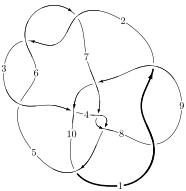
\includegraphics[width=112pt]{../../../GIT/diagram.site/Diagrams/png/177_10_93.png}\\
\ \ \ A knot diagram\footnotemark}&
\allowdisplaybreaks
\textbf{Linearized knot diagam} \\
\cline{2-2}
 &
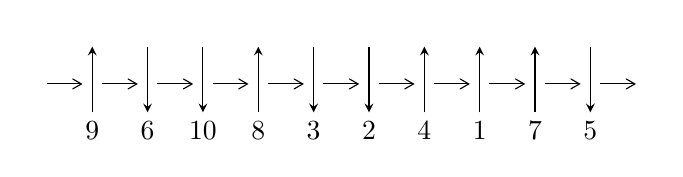
\begin{tikzpicture}[x=20pt, y=17pt]
	% nodes
	\node (C0) at (0, 0) {};
	\node (C1) at (1, 0) {};
	\node (C1U) at (1, +1) {};
	\node (C1D) at (1, -1) {9};

	\node (C2) at (2, 0) {};
	\node (C2U) at (2, +1) {};
	\node (C2D) at (2, -1) {6};

	\node (C3) at (3, 0) {};
	\node (C3U) at (3, +1) {};
	\node (C3D) at (3, -1) {10};

	\node (C4) at (4, 0) {};
	\node (C4U) at (4, +1) {};
	\node (C4D) at (4, -1) {8};

	\node (C5) at (5, 0) {};
	\node (C5U) at (5, +1) {};
	\node (C5D) at (5, -1) {3};

	\node (C6) at (6, 0) {};
	\node (C6U) at (6, +1) {};
	\node (C6D) at (6, -1) {2};

	\node (C7) at (7, 0) {};
	\node (C7U) at (7, +1) {};
	\node (C7D) at (7, -1) {4};

	\node (C8) at (8, 0) {};
	\node (C8U) at (8, +1) {};
	\node (C8D) at (8, -1) {1};

	\node (C9) at (9, 0) {};
	\node (C9U) at (9, +1) {};
	\node (C9D) at (9, -1) {7};

	\node (C10) at (10, 0) {};
	\node (C10U) at (10, +1) {};
	\node (C10D) at (10, -1) {5};
	\node (C11) at (11, 0) {};

	% arrows
	\draw[->,>={angle 60}]
	(C0) edge (C1) (C1) edge (C2) (C2) edge (C3) (C3) edge (C4) (C4) edge (C5) (C5) edge (C6) (C6) edge (C7) (C7) edge (C8) (C8) edge (C9) (C9) edge (C10) (C10) edge (C11) ;	\draw[->,>=stealth]
	(C1D) edge (C1U) (C2U) edge (C2D) (C3U) edge (C3D) (C4D) edge (C4U) (C5U) edge (C5D) (C6U) edge (C6D) (C7D) edge (C7U) (C8D) edge (C8U) (C9D) edge (C9U) (C10U) edge (C10D) ;
	\end{tikzpicture} \\
\hhline{~~} \\& 
\textbf{Solving Sequence} \\ \cline{2-2} 
 &
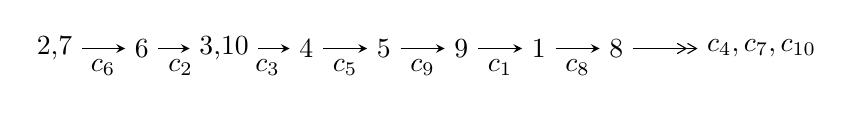
\begin{tikzpicture}[x=28pt, y=7pt]
	% node
	\node (A0) at (-1/8, 0) {2,7};
	\node (A1) at (1, 0) {6};
	\node (A2) at (33/16, 0) {3,10};
	\node (A3) at (25/8, 0) {4};
	\node (A4) at (33/8, 0) {5};
	\node (A5) at (41/8, 0) {9};
	\node (A6) at (49/8, 0) {1};
	\node (A7) at (57/8, 0) {8};
	\node (C1) at (1/2, -1) {$c_{6}$};
	\node (C2) at (3/2, -1) {$c_{2}$};
	\node (C3) at (21/8, -1) {$c_{3}$};
	\node (C4) at (29/8, -1) {$c_{5}$};
	\node (C5) at (37/8, -1) {$c_{9}$};
	\node (C6) at (45/8, -1) {$c_{1}$};
	\node (C7) at (53/8, -1) {$c_{8}$};
	\node (A8) at (9, 0) {$c_{4},c_{7},c_{10}$};

	% edge
	\draw[->,>=stealth]	
	(A0) edge (A1) (A1) edge (A2) (A2) edge (A3) (A3) edge (A4) (A4) edge (A5) (A5) edge (A6) (A6) edge (A7) ;
	\draw[->>,>={angle 60}]	
	(A7) edge (A8);
\end{tikzpicture} \\ 

\end{tabular} \\

\footnotetext{
The image of knot diagram is generated by the software ``\textbf{Draw programme}" developed by Andrew Bartholomew(\url{http://www.layer8.co.uk/maths/draw/index.htm\#Running-draw}), where we modified some parts for our purpose(\url{https://github.com/CATsTAILs/LinksPainter}).
}\phantom \\ \newline 
\centering \textbf{Ideals for irreducible components\footnotemark of $X_{\text{par}}$} 
 
\begin{align*}
I^u_{1}&=\langle 
-1.48497\times10^{17} u^{34}-2.74759\times10^{17} u^{33}+\cdots+2.14980\times10^{17} b+3.71507\times10^{17},\\
\phantom{I^u_{1}}&\phantom{= \langle  }2.04229\times10^{17} u^{34}+3.73430\times10^{17} u^{33}+\cdots+2.14980\times10^{17} a-2.36397\times10^{17},\;u^{35}+2 u^{34}+\cdots-2 u-1\rangle \\
I^u_{2}&=\langle 
3 b+u+2,\;3 a-2 u-1,\;u^2+u+1\rangle \\
\\
\end{align*}
\raggedright * 2 irreducible components of $\dim_{\mathbb{C}}=0$, with total 37 representations.\\
\footnotetext{All coefficients of polynomials are rational numbers. But the coefficients are sometimes approximated in decimal forms when there is not enough margin.}
\newpage
\renewcommand{\arraystretch}{1}
\centering \section*{I. $I^u_{1}= \langle -1.48\times10^{17} u^{34}-2.75\times10^{17} u^{33}+\cdots+2.15\times10^{17} b+3.72\times10^{17},\;2.04\times10^{17} u^{34}+3.73\times10^{17} u^{33}+\cdots+2.15\times10^{17} a-2.36\times10^{17},\;u^{35}+2 u^{34}+\cdots-2 u-1 \rangle$}
\flushleft \textbf{(i) Arc colorings}\\
\begin{tabular}{m{7pt} m{180pt} m{7pt} m{180pt} }
\flushright $a_{2}=$&$\begin{pmatrix}0\\u\end{pmatrix}$ \\
\flushright $a_{7}=$&$\begin{pmatrix}1\\0\end{pmatrix}$ \\
\flushright $a_{6}=$&$\begin{pmatrix}1\\- u^2\end{pmatrix}$ \\
\flushright $a_{3}=$&$\begin{pmatrix}- u\\u^3+u\end{pmatrix}$ \\
\flushright $a_{10}=$&$\begin{pmatrix}-0.949992 u^{34}-1.73705 u^{33}+\cdots+6.42492 u+1.09963\\0.690747 u^{34}+1.27807 u^{33}+\cdots-1.42690 u-1.72810\end{pmatrix}$ \\
\flushright $a_{4}=$&$\begin{pmatrix}0.300462 u^{34}+0.653361 u^{33}+\cdots+0.171322 u-0.984845\\0.369645 u^{34}+0.462967 u^{33}+\cdots-2.38683 u-0.219453\end{pmatrix}$ \\
\flushright $a_{5}=$&$\begin{pmatrix}u^2+1\\- u^4-2 u^2\end{pmatrix}$ \\
\flushright $a_{9}=$&$\begin{pmatrix}-1.64074 u^{34}-3.01512 u^{33}+\cdots+7.85182 u+2.82773\\0.690747 u^{34}+1.27807 u^{33}+\cdots-1.42690 u-1.72810\end{pmatrix}$ \\
\flushright $a_{1}=$&$\begin{pmatrix}-1.39270 u^{34}-2.59706 u^{33}+\cdots+7.17623 u+2.38722\\0.569891 u^{34}+1.15346 u^{33}+\cdots-0.0996613 u-1.67732\end{pmatrix}$ \\
\flushright $a_{8}=$&$\begin{pmatrix}-0.604507 u^{34}-1.03705 u^{33}+\cdots+1.81017 u+1.15186\\0.344862 u^{34}+0.434712 u^{33}+\cdots-1.72091 u-0.338982\end{pmatrix}$\\&\end{tabular}
\flushleft \textbf{(ii) Obstruction class $= -1$}\\~\\
\flushleft \textbf{(iii) Cusp Shapes $= -\frac{43902992914495201}{128987874023997969} u^{34}-\frac{378946062727999073}{214979790039996615} u^{33}+\cdots-\frac{1287205910561212151}{214979790039996615} u+\frac{3437895448731260974}{644939370119989845}$}\\~\\
\newpage\renewcommand{\arraystretch}{1}
\flushleft \textbf{(iv) u-Polynomials at the component}\newline \\
\begin{tabular}{m{50pt}|m{274pt}}
Crossings & \hspace{64pt}u-Polynomials at each crossing \\
\hline $$\begin{aligned}c_{1},c_{8}\end{aligned}$$&$\begin{aligned}
&u^{35}+3 u^{34}+\cdots+5 u-9
\end{aligned}$\\
\hline $$\begin{aligned}c_{2},c_{5},c_{6}\end{aligned}$$&$\begin{aligned}
&u^{35}-2 u^{34}+\cdots-2 u+1
\end{aligned}$\\
\hline $$\begin{aligned}c_{3}\end{aligned}$$&$\begin{aligned}
&u^{35}+3 u^{34}+\cdots-60 u+36
\end{aligned}$\\
\hline $$\begin{aligned}c_{4},c_{7}\end{aligned}$$&$\begin{aligned}
&u^{35}-2 u^{34}+\cdots+2 u-1
\end{aligned}$\\
\hline $$\begin{aligned}c_{9}\end{aligned}$$&$\begin{aligned}
&3(3 u^{35}+2 u^{34}+\cdots+2024 u+529)
\end{aligned}$\\
\hline $$\begin{aligned}c_{10}\end{aligned}$$&$\begin{aligned}
&3(3 u^{35}+13 u^{34}+\cdots-793 u+173)
\end{aligned}$\\
\hline
\end{tabular}\\~\\
\newpage\renewcommand{\arraystretch}{1}
\flushleft \textbf{(v) Riley Polynomials at the component}\newline \\
\begin{tabular}{m{50pt}|m{274pt}}
Crossings & \hspace{64pt}Riley Polynomials at each crossing \\
\hline $$\begin{aligned}c_{1},c_{8}\end{aligned}$$&$\begin{aligned}
&y^{35}-31 y^{34}+\cdots+439 y-81
\end{aligned}$\\
\hline $$\begin{aligned}c_{2},c_{5},c_{6}\end{aligned}$$&$\begin{aligned}
&y^{35}+36 y^{34}+\cdots-8 y-1
\end{aligned}$\\
\hline $$\begin{aligned}c_{3}\end{aligned}$$&$\begin{aligned}
&y^{35}+15 y^{34}+\cdots-8136 y-1296
\end{aligned}$\\
\hline $$\begin{aligned}c_{4},c_{7}\end{aligned}$$&$\begin{aligned}
&y^{35}-24 y^{34}+\cdots-8 y-1
\end{aligned}$\\
\hline $$\begin{aligned}c_{9}\end{aligned}$$&$\begin{aligned}
&9(9 y^{35}-280 y^{34}+\cdots+2073680 y-279841)
\end{aligned}$\\
\hline $$\begin{aligned}c_{10}\end{aligned}$$&$\begin{aligned}
&9(9 y^{35}+137 y^{34}+\cdots+24387 y-29929)
\end{aligned}$\\
\hline
\end{tabular}\\~\\
\newpage\flushleft \textbf{(vi) Complex Volumes and Cusp Shapes}
$$\begin{array}{c|c|c}  
\text{Solutions to }I^u_{1}& \I (\text{vol} + \sqrt{-1}CS) & \text{Cusp shape}\\
 \hline 
\begin{aligned}
u &= -0.797949 + 0.618523 I \\
a &= \phantom{-}0.441661 - 0.524170 I \\
b &= \phantom{-}1.31533 + 0.64336 I\end{aligned}
 & \phantom{-}7.15893 + 9.08856 I & \phantom{-}5.28395 - 6.85993 I \\ \hline\begin{aligned}
u &= -0.797949 - 0.618523 I \\
a &= \phantom{-}0.441661 + 0.524170 I \\
b &= \phantom{-}1.31533 - 0.64336 I\end{aligned}
 & \phantom{-}7.15893 - 9.08856 I & \phantom{-}5.28395 + 6.85993 I \\ \hline\begin{aligned}
u &= \phantom{-}0.319146 + 0.974832 I \\
a &= -0.0301867 + 0.0609842 I \\
b &= -0.142675 + 0.589069 I\end{aligned}
 & \phantom{-}0.84892 - 2.27938 I & -3.03865 + 4.27236 I \\ \hline\begin{aligned}
u &= \phantom{-}0.319146 - 0.974832 I \\
a &= -0.0301867 - 0.0609842 I \\
b &= -0.142675 - 0.589069 I\end{aligned}
 & \phantom{-}0.84892 + 2.27938 I & -3.03865 - 4.27236 I \\ \hline\begin{aligned}
u &= -0.883803 + 0.527645 I \\
a &= -0.151524 - 0.698091 I \\
b &= \phantom{-}1.074450 - 0.184550 I\end{aligned}
 & \phantom{-}6.81152 - 3.53470 I & \phantom{-}6.64372 + 2.46356 I \\ \hline\begin{aligned}
u &= -0.883803 - 0.527645 I \\
a &= -0.151524 + 0.698091 I \\
b &= \phantom{-}1.074450 + 0.184550 I\end{aligned}
 & \phantom{-}6.81152 + 3.53470 I & \phantom{-}6.64372 - 2.46356 I \\ \hline\begin{aligned}
u &= \phantom{-}0.890046 + 0.661300 I \\
a &= -0.138488 - 0.436432 I \\
b &= -0.961888 + 0.317896 I\end{aligned}
 & \phantom{-}2.19099 - 3.04973 I & \phantom{-}6.83792 + 5.73006 I \\ \hline\begin{aligned}
u &= \phantom{-}0.890046 - 0.661300 I \\
a &= -0.138488 + 0.436432 I \\
b &= -0.961888 - 0.317896 I\end{aligned}
 & \phantom{-}2.19099 + 3.04973 I & \phantom{-}6.83792 - 5.73006 I \\ \hline\begin{aligned}
u &= -0.485797 + 0.446415 I \\
a &= -1.54295 + 0.61782 I \\
b &= -0.767630 - 0.733842 I\end{aligned}
 & \phantom{-}1.92901 + 4.20671 I & \phantom{-}2.61467 - 7.67969 I \\ \hline\begin{aligned}
u &= -0.485797 - 0.446415 I \\
a &= -1.54295 - 0.61782 I \\
b &= -0.767630 + 0.733842 I\end{aligned}
 & \phantom{-}1.92901 - 4.20671 I & \phantom{-}2.61467 + 7.67969 I\\
 \hline 
 \end{array}$$\newpage$$\begin{array}{c|c|c}  
\text{Solutions to }I^u_{1}& \I (\text{vol} + \sqrt{-1}CS) & \text{Cusp shape}\\
 \hline 
\begin{aligned}
u &= \phantom{-}0.177701 + 0.568169 I \\
a &= \phantom{-}0.88046 + 2.71785 I \\
b &= \phantom{-}0.844702 + 0.231272 I\end{aligned}
 & \phantom{-}5.61974 - 1.75521 I & \phantom{-}9.80898 + 3.99717 I \\ \hline\begin{aligned}
u &= \phantom{-}0.177701 - 0.568169 I \\
a &= \phantom{-}0.88046 - 2.71785 I \\
b &= \phantom{-}0.844702 - 0.231272 I\end{aligned}
 & \phantom{-}5.61974 + 1.75521 I & \phantom{-}9.80898 - 3.99717 I \\ \hline\begin{aligned}
u &= \phantom{-}0.518141 + 0.274512 I \\
a &= \phantom{-}0.865516 + 0.243501 I \\
b &= \phantom{-}0.321578 - 0.365013 I\end{aligned}
 & -1.063790 - 0.837639 I & -5.45708 + 2.88305 I \\ \hline\begin{aligned}
u &= \phantom{-}0.518141 - 0.274512 I \\
a &= \phantom{-}0.865516 - 0.243501 I \\
b &= \phantom{-}0.321578 + 0.365013 I\end{aligned}
 & -1.063790 + 0.837639 I & -5.45708 - 2.88305 I \\ \hline\begin{aligned}
u &= -0.07117 + 1.42730 I \\
a &= -2.02061 + 1.49459 I \\
b &= -1.94022 + 1.12557 I\end{aligned}
 & \phantom{-}7.48516 + 0.26471 I & \phantom{-}8.26333 + 0. I\phantom{ +0.000000I} \\ \hline\begin{aligned}
u &= -0.07117 - 1.42730 I \\
a &= -2.02061 - 1.49459 I \\
b &= -1.94022 - 1.12557 I\end{aligned}
 & \phantom{-}7.48516 - 0.26471 I & \phantom{-}8.26333 + 0. I\phantom{ +0.000000I} \\ \hline\begin{aligned}
u &= \phantom{-}0.13283 + 1.44979 I \\
a &= \phantom{-}1.51691 + 0.10394 I \\
b &= \phantom{-}0.950697 - 0.074489 I\end{aligned}
 & \phantom{-}4.57837 - 3.04741 I & \phantom{-0.000000 } 0 \\ \hline\begin{aligned}
u &= \phantom{-}0.13283 - 1.44979 I \\
a &= \phantom{-}1.51691 - 0.10394 I \\
b &= \phantom{-}0.950697 + 0.074489 I\end{aligned}
 & \phantom{-}4.57837 + 3.04741 I & \phantom{-0.000000 } 0 \\ \hline\begin{aligned}
u &= -0.379190 + 0.370732 I \\
a &= \phantom{-}0.133491 + 0.548267 I \\
b &= -0.738044 + 0.811910 I\end{aligned}
 & \phantom{-}1.88873 - 1.15770 I & \phantom{-}2.26234 - 1.26872 I \\ \hline\begin{aligned}
u &= -0.379190 - 0.370732 I \\
a &= \phantom{-}0.133491 - 0.548267 I \\
b &= -0.738044 - 0.811910 I\end{aligned}
 & \phantom{-}1.88873 + 1.15770 I & \phantom{-}2.26234 + 1.26872 I\\
 \hline 
 \end{array}$$\newpage$$\begin{array}{c|c|c}  
\text{Solutions to }I^u_{1}& \I (\text{vol} + \sqrt{-1}CS) & \text{Cusp shape}\\
 \hline 
\begin{aligned}
u &= -0.03075 + 1.47995 I \\
a &= -1.46910 - 0.67161 I \\
b &= -1.29110 - 1.51306 I\end{aligned}
 & \phantom{-}7.85287 + 1.23959 I & \phantom{-0.000000 } 0 \\ \hline\begin{aligned}
u &= -0.03075 - 1.47995 I \\
a &= -1.46910 + 0.67161 I \\
b &= -1.29110 + 1.51306 I\end{aligned}
 & \phantom{-}7.85287 - 1.23959 I & \phantom{-0.000000 } 0 \\ \hline\begin{aligned}
u &= -0.13948 + 1.49938 I \\
a &= -1.99280 - 0.18614 I \\
b &= -1.072190 - 0.508436 I\end{aligned}
 & \phantom{-}8.34974 + 6.42549 I & \phantom{-0.000000 } 0 \\ \hline\begin{aligned}
u &= -0.13948 - 1.49938 I \\
a &= -1.99280 + 0.18614 I \\
b &= -1.072190 + 0.508436 I\end{aligned}
 & \phantom{-}8.34974 - 6.42549 I & \phantom{-0.000000 } 0 \\ \hline\begin{aligned}
u &= \phantom{-}0.04304 + 1.53065 I \\
a &= \phantom{-}1.29303 + 0.78816 I \\
b &= \phantom{-}0.854691 - 0.412838 I\end{aligned}
 & \phantom{-}12.61950 - 2.50960 I & \phantom{-}11.52662 + 0. I\phantom{ +0.000000I} \\ \hline\begin{aligned}
u &= \phantom{-}0.04304 - 1.53065 I \\
a &= \phantom{-}1.29303 - 0.78816 I \\
b &= \phantom{-}0.854691 + 0.412838 I\end{aligned}
 & \phantom{-}12.61950 + 2.50960 I & \phantom{-}11.52662 + 0. I\phantom{ +0.000000I} \\ \hline\begin{aligned}
u &= -0.26639 + 1.57422 I \\
a &= \phantom{-}1.85469 - 0.10458 I \\
b &= \phantom{-}1.70003 + 0.90521 I\end{aligned}
 & \phantom{-}14.3602 + 13.0165 I & \phantom{-0.000000 } 0 \\ \hline\begin{aligned}
u &= -0.26639 - 1.57422 I \\
a &= \phantom{-}1.85469 + 0.10458 I \\
b &= \phantom{-}1.70003 - 0.90521 I\end{aligned}
 & \phantom{-}14.3602 - 13.0165 I & \phantom{-0.000000 } 0 \\ \hline\begin{aligned}
u &= -0.171298 + 0.343458 I \\
a &= -0.06814 + 1.97682 I \\
b &= -0.847997 - 0.510070 I\end{aligned}
 & \phantom{-}1.76589 + 0.63046 I & \phantom{-}5.20787 + 1.46477 I \\ \hline\begin{aligned}
u &= -0.171298 - 0.343458 I \\
a &= -0.06814 - 1.97682 I \\
b &= -0.847997 + 0.510070 I\end{aligned}
 & \phantom{-}1.76589 - 0.63046 I & \phantom{-}5.20787 - 1.46477 I\\
 \hline 
 \end{array}$$\newpage$$\begin{array}{c|c|c}  
\text{Solutions to }I^u_{1}& \I (\text{vol} + \sqrt{-1}CS) & \text{Cusp shape}\\
 \hline 
\begin{aligned}
u &= \phantom{-}0.27157 + 1.59599 I \\
a &= -1.399030 - 0.062212 I \\
b &= -1.34067 + 0.82337 I\end{aligned}
 & \phantom{-}9.65156 - 7.25912 I & \phantom{-0.000000 } 0 \\ \hline\begin{aligned}
u &= \phantom{-}0.27157 - 1.59599 I \\
a &= -1.399030 + 0.062212 I \\
b &= -1.34067 - 0.82337 I\end{aligned}
 & \phantom{-}9.65156 + 7.25912 I & \phantom{-0.000000 } 0 \\ \hline\begin{aligned}
u &= -0.31084 + 1.58997 I \\
a &= \phantom{-}0.998238 - 0.474581 I \\
b &= \phantom{-}1.142220 + 0.398928 I\end{aligned}
 & \phantom{-}13.76820 + 0.95076 I & \phantom{-0.000000 } 0 \\ \hline\begin{aligned}
u &= -0.31084 - 1.58997 I \\
a &= \phantom{-}0.998238 + 0.474581 I \\
b &= \phantom{-}1.142220 - 0.398928 I\end{aligned}
 & \phantom{-}13.76820 - 0.95076 I & \phantom{-0.000000 } 0 \\ \hline\begin{aligned}
u &= \phantom{-}0.368379\phantom{ +0.000000I} \\
a &= -0.675672\phantom{ +0.000000I} \\
b &= \phantom{-}2.46408\phantom{ +0.000000I}\end{aligned}
 & \phantom{-}3.85534\phantom{ +0.000000I} & -11.8900\phantom{ +0.000000I}\\
 \hline 
 \end{array}$$\newpage\newpage\renewcommand{\arraystretch}{1}
\centering \section*{II. $I^u_{2}= \langle 3 b+u+2,\;3 a-2 u-1,\;u^2+u+1 \rangle$}
\flushleft \textbf{(i) Arc colorings}\\
\begin{tabular}{m{7pt} m{180pt} m{7pt} m{180pt} }
\flushright $a_{2}=$&$\begin{pmatrix}0\\u\end{pmatrix}$ \\
\flushright $a_{7}=$&$\begin{pmatrix}1\\0\end{pmatrix}$ \\
\flushright $a_{6}=$&$\begin{pmatrix}1\\u+1\end{pmatrix}$ \\
\flushright $a_{3}=$&$\begin{pmatrix}- u\\u+1\end{pmatrix}$ \\
\flushright $a_{10}=$&$\begin{pmatrix}\frac{2}{3} u+\frac{1}{3}\\-\frac{1}{3} u-\frac{2}{3}\end{pmatrix}$ \\
\flushright $a_{4}=$&$\begin{pmatrix}- u\\u+1\end{pmatrix}$ \\
\flushright $a_{5}=$&$\begin{pmatrix}- u\\u+2\end{pmatrix}$ \\
\flushright $a_{9}=$&$\begin{pmatrix}u+1\\-\frac{1}{3} u-\frac{2}{3}\end{pmatrix}$ \\
\flushright $a_{1}=$&$\begin{pmatrix}u+1\\\frac{2}{3} u-\frac{2}{3}\end{pmatrix}$ \\
\flushright $a_{8}=$&$\begin{pmatrix}0\\- u\end{pmatrix}$\\&\end{tabular}
\flushleft \textbf{(ii) Obstruction class $= 1$}\\~\\
\flushleft \textbf{(iii) Cusp Shapes $= -\frac{4}{3} u+5$}\\~\\
\newpage\renewcommand{\arraystretch}{1}
\flushleft \textbf{(iv) u-Polynomials at the component}\newline \\
\begin{tabular}{m{50pt}|m{274pt}}
Crossings & \hspace{64pt}u-Polynomials at each crossing \\
\hline $$\begin{aligned}c_{1}\end{aligned}$$&$\begin{aligned}
&(u-1)^2
\end{aligned}$\\
\hline $$\begin{aligned}c_{2},c_{7}\end{aligned}$$&$\begin{aligned}
&u^2- u+1
\end{aligned}$\\
\hline $$\begin{aligned}c_{3}\end{aligned}$$&$\begin{aligned}
&u^2
\end{aligned}$\\
\hline $$\begin{aligned}c_{4},c_{5},c_{6}\end{aligned}$$&$\begin{aligned}
&u^2+u+1
\end{aligned}$\\
\hline $$\begin{aligned}c_{8}\end{aligned}$$&$\begin{aligned}
&(u+1)^2
\end{aligned}$\\
\hline $$\begin{aligned}c_{9}\end{aligned}$$&$\begin{aligned}
&3(3 u^2-3 u+1)
\end{aligned}$\\
\hline $$\begin{aligned}c_{10}\end{aligned}$$&$\begin{aligned}
&3(3 u^2+1)
\end{aligned}$\\
\hline
\end{tabular}\\~\\
\newpage\renewcommand{\arraystretch}{1}
\flushleft \textbf{(v) Riley Polynomials at the component}\newline \\
\begin{tabular}{m{50pt}|m{274pt}}
Crossings & \hspace{64pt}Riley Polynomials at each crossing \\
\hline $$\begin{aligned}c_{1},c_{8}\end{aligned}$$&$\begin{aligned}
&(y-1)^2
\end{aligned}$\\
\hline $$\begin{aligned}c_{2},c_{4},c_{5}\\c_{6},c_{7}\end{aligned}$$&$\begin{aligned}
&y^2+y+1
\end{aligned}$\\
\hline $$\begin{aligned}c_{3}\end{aligned}$$&$\begin{aligned}
&y^2
\end{aligned}$\\
\hline $$\begin{aligned}c_{9}\end{aligned}$$&$\begin{aligned}
&9(9 y^2-3 y+1)
\end{aligned}$\\
\hline $$\begin{aligned}c_{10}\end{aligned}$$&$\begin{aligned}
&9(3 y+1)^2
\end{aligned}$\\
\hline
\end{tabular}\\~\\
\newpage\flushleft \textbf{(vi) Complex Volumes and Cusp Shapes}
$$\begin{array}{c|c|c}  
\text{Solutions to }I^u_{2}& \I (\text{vol} + \sqrt{-1}CS) & \text{Cusp shape}\\
 \hline 
\begin{aligned}
u &= -0.500000 + 0.866025 I \\
a &= \phantom{-0.000000 -}0.577350 I \\
b &= -0.500000 - 0.288675 I\end{aligned}
 & \phantom{-}1.64493 + 2.02988 I & \phantom{-}5.66667 - 1.15470 I \\ \hline\begin{aligned}
u &= -0.500000 - 0.866025 I \\
a &= \phantom{-0.000000 } -0.577350 I \\
b &= -0.500000 + 0.288675 I\end{aligned}
 & \phantom{-}1.64493 - 2.02988 I & \phantom{-}5.66667 + 1.15470 I\\
 \hline 
 \end{array}$$\newpage
\newpage\renewcommand{\arraystretch}{1}
\centering \section*{ III. u-Polynomials}
\begin{tabular}{m{50pt}|m{274pt}}
Crossings & \hspace{64pt}u-Polynomials at each crossing \\
\hline $$\begin{aligned}c_{1}\end{aligned}$$&$\begin{aligned}
&((u-1)^2)(u^{35}+3 u^{34}+\cdots+5 u-9)
\end{aligned}$\\
\hline $$\begin{aligned}c_{2}\end{aligned}$$&$\begin{aligned}
&(u^2- u+1)(u^{35}-2 u^{34}+\cdots-2 u+1)
\end{aligned}$\\
\hline $$\begin{aligned}c_{3}\end{aligned}$$&$\begin{aligned}
&u^2(u^{35}+3 u^{34}+\cdots-60 u+36)
\end{aligned}$\\
\hline $$\begin{aligned}c_{4}\end{aligned}$$&$\begin{aligned}
&(u^2+u+1)(u^{35}-2 u^{34}+\cdots+2 u-1)
\end{aligned}$\\
\hline $$\begin{aligned}c_{5},c_{6}\end{aligned}$$&$\begin{aligned}
&(u^2+u+1)(u^{35}-2 u^{34}+\cdots-2 u+1)
\end{aligned}$\\
\hline $$\begin{aligned}c_{7}\end{aligned}$$&$\begin{aligned}
&(u^2- u+1)(u^{35}-2 u^{34}+\cdots+2 u-1)
\end{aligned}$\\
\hline $$\begin{aligned}c_{8}\end{aligned}$$&$\begin{aligned}
&((u+1)^2)(u^{35}+3 u^{34}+\cdots+5 u-9)
\end{aligned}$\\
\hline $$\begin{aligned}c_{9}\end{aligned}$$&$\begin{aligned}
&9(3 u^2-3 u+1)(3 u^{35}+2 u^{34}+\cdots+2024 u+529)
\end{aligned}$\\
\hline $$\begin{aligned}c_{10}\end{aligned}$$&$\begin{aligned}
&9(3 u^2+1)(3 u^{35}+13 u^{34}+\cdots-793 u+173)
\end{aligned}$\\
\hline
\end{tabular}\newpage\renewcommand{\arraystretch}{1}
\centering \section*{ IV. Riley Polynomials}
\begin{tabular}{m{50pt}|m{274pt}}
Crossings & \hspace{64pt}Riley Polynomials at each crossing \\
\hline $$\begin{aligned}c_{1},c_{8}\end{aligned}$$&$\begin{aligned}
&((y-1)^2)(y^{35}-31 y^{34}+\cdots+439 y-81)
\end{aligned}$\\
\hline $$\begin{aligned}c_{2},c_{5},c_{6}\end{aligned}$$&$\begin{aligned}
&(y^2+y+1)(y^{35}+36 y^{34}+\cdots-8 y-1)
\end{aligned}$\\
\hline $$\begin{aligned}c_{3}\end{aligned}$$&$\begin{aligned}
&y^2(y^{35}+15 y^{34}+\cdots-8136 y-1296)
\end{aligned}$\\
\hline $$\begin{aligned}c_{4},c_{7}\end{aligned}$$&$\begin{aligned}
&(y^2+y+1)(y^{35}-24 y^{34}+\cdots-8 y-1)
\end{aligned}$\\
\hline $$\begin{aligned}c_{9}\end{aligned}$$&$\begin{aligned}
&81(9 y^2-3 y+1)(9 y^{35}-280 y^{34}+\cdots+2073680 y-279841)
\end{aligned}$\\
\hline $$\begin{aligned}c_{10}\end{aligned}$$&$\begin{aligned}
&81(3 y+1)^2(9 y^{35}+137 y^{34}+\cdots+24387 y-29929)
\end{aligned}$\\
\hline
\end{tabular}
\vskip 2pc
\end{document}